\chapter{Résultats et discussion}
Ce chapitre discute des résultats obtenus par ce projet.

\section{Description du bras robotique Ovis}
La définition du bras représente de manière fidèle le bras physique. Les membrures et joints sont positionnés adéquatement et leurs limites sont bien définies. La description est modulaire puisque la géométrie du bras est appelée à être modifiée au cours des prochaines années.

\section{Simulation}
\subsection{Simulateur industriel}
La simulation du manipulateur par le simulateur industriel est efficace pour effectuer le développement d'un algorithme. Toutefois, l'affichage des mouvement dans RViz est légèrement saccadé, ceci semble être un défaut provenant du simulateur industriel plutôt que de l'algorithme développé. Afin de valider cette hypothèse, un algorithme de contrôle préexistant fut testé et la simulation répondait de manière similaire.

\subsection{Simulateur Gazebo}
La simulation du manipulateur avec Gazebo est maintenant complété. Toutefois, la pince Robotiq apparaît mais n'est pas simulé adéquatement tel que mentionné à la section \ref{subsec:pince_gazebo}. L'ajout d'un contrôleur logiciel réglerait ce problème, mais puisqu'il n'y a pas de valeur ajoutée pour ce projet la pince restera simulée ainsi. La figure \ref{fig:gazebo_sim_rviz} montre la visualisation du bras dans RViz, lors de la simulation par Gazebo. On aperçoit l'image de la caméra au poignet aussi générée par Gazebo.
Une vidéo de la simulation est disponible en ligne à \url{https://youtu.be/ZcYvDAnuGzY}.

\begin{figure}
    \centering
    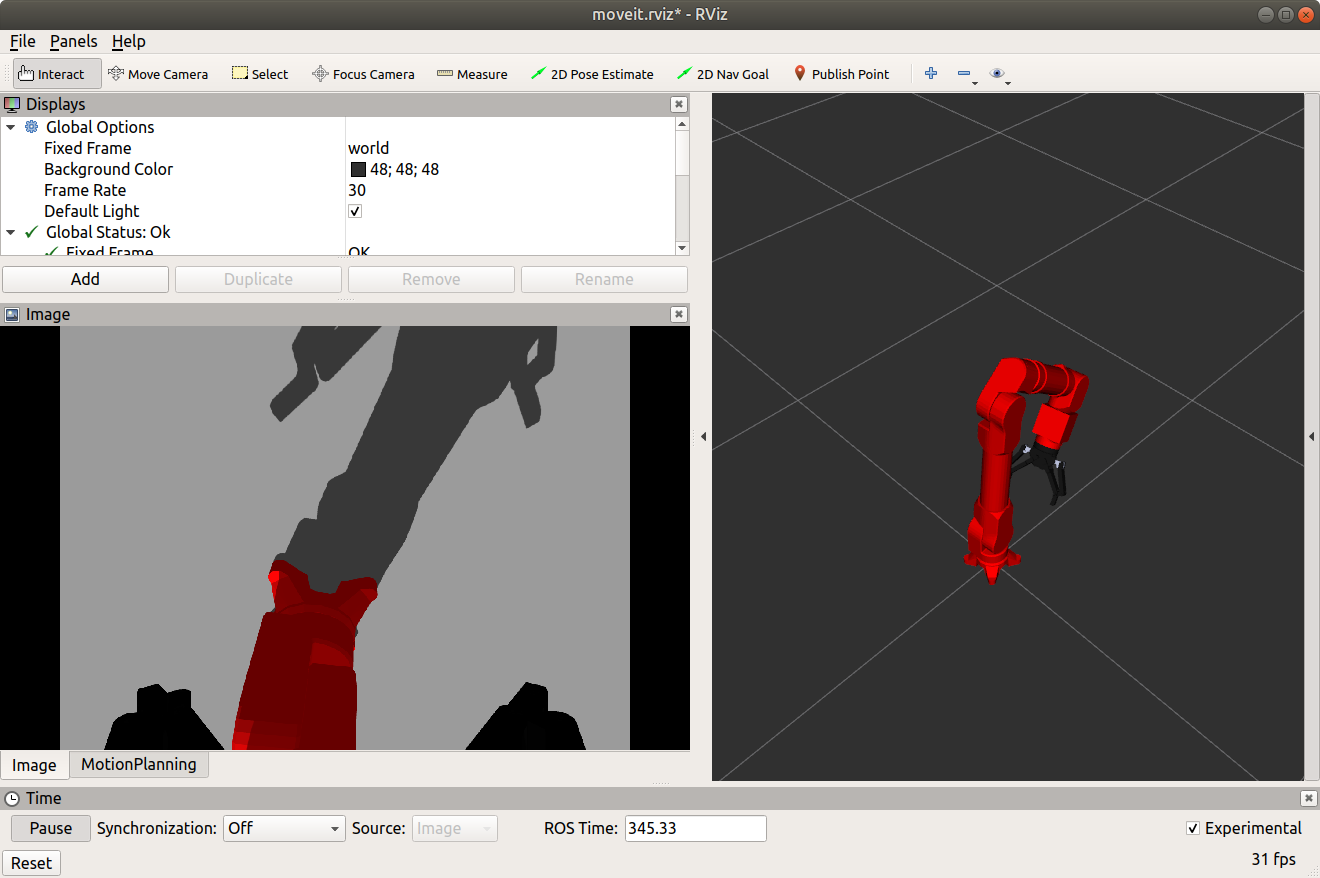
\includegraphics[%scale=0.35
                    width=\textwidth]{Figures/gazebo_sim_rviz.png}
    \caption{Ovis et sa caméra simulée par Gazebo et visualisée dans RViz}
    \label{fig:gazebo_sim_rviz}
\end{figure}


\section{Algorithme}
L'algorithme de contrôle en C++ est qualitativement plus rapide que le prototype précédent. Afin de valider que l'algorithme est, tel que souhaité, c'est à dire simple d'utilisation pour un opérateur n'ayant aucune expérience préalable, l'algorithme fut testé par quelques personnes externes au projet. Il n'y a eu aucun commentaires négatifs, l'expérience fut appréciée de tous. L'algorithme comporte toutefois certaines lacunes. Tout comme un robot industriel en mode \emph{jog} qui effectue un mouvement linéaire, lorsque deux axes se trouvent à être parallèles le bras arrive à une singularité. L'algorithme ne gère pas ce cas particulier. Aussi, lorsque la pince du robot approche la limite de la zone de travail, le robot peut être plus difficile à manipuler puisqu'il perd généralement %là-aussi 
un degré de liberté. Une solution envisagée pour palier ce problème est d'ajouter un contrôleur qui plutôt que de commander directement le système d'axes de référence, enverrait un vecteur afin de pousser/tirer virtuellement sur le système d'axes à l'outil. Finalement, malgré que l'algorithme permette au bras d'éviter les collisions avec lui-même et les objets connus de son environnement, celui-ci dépend de capteurs externes au bras. Une collision est possible entre le bras et un élément inconnu de l'environnement. Un événement de ce type n'est pas prévisible, mais l'algorithme pourrait être amélioré afin de tenir compte des capteurs de forces présent dans les actuateurs du bras et ainsi éviter d'endommager le manipulateur. En résumé, l'algorithme répond bien aux critères énoncés en début de projet et ce malgré qu'il ne soit fonctionnel que sur une plage réduite de l'enveloppe totale de travail accessible par le manipulateur.

\begin{figure}
    \centering
    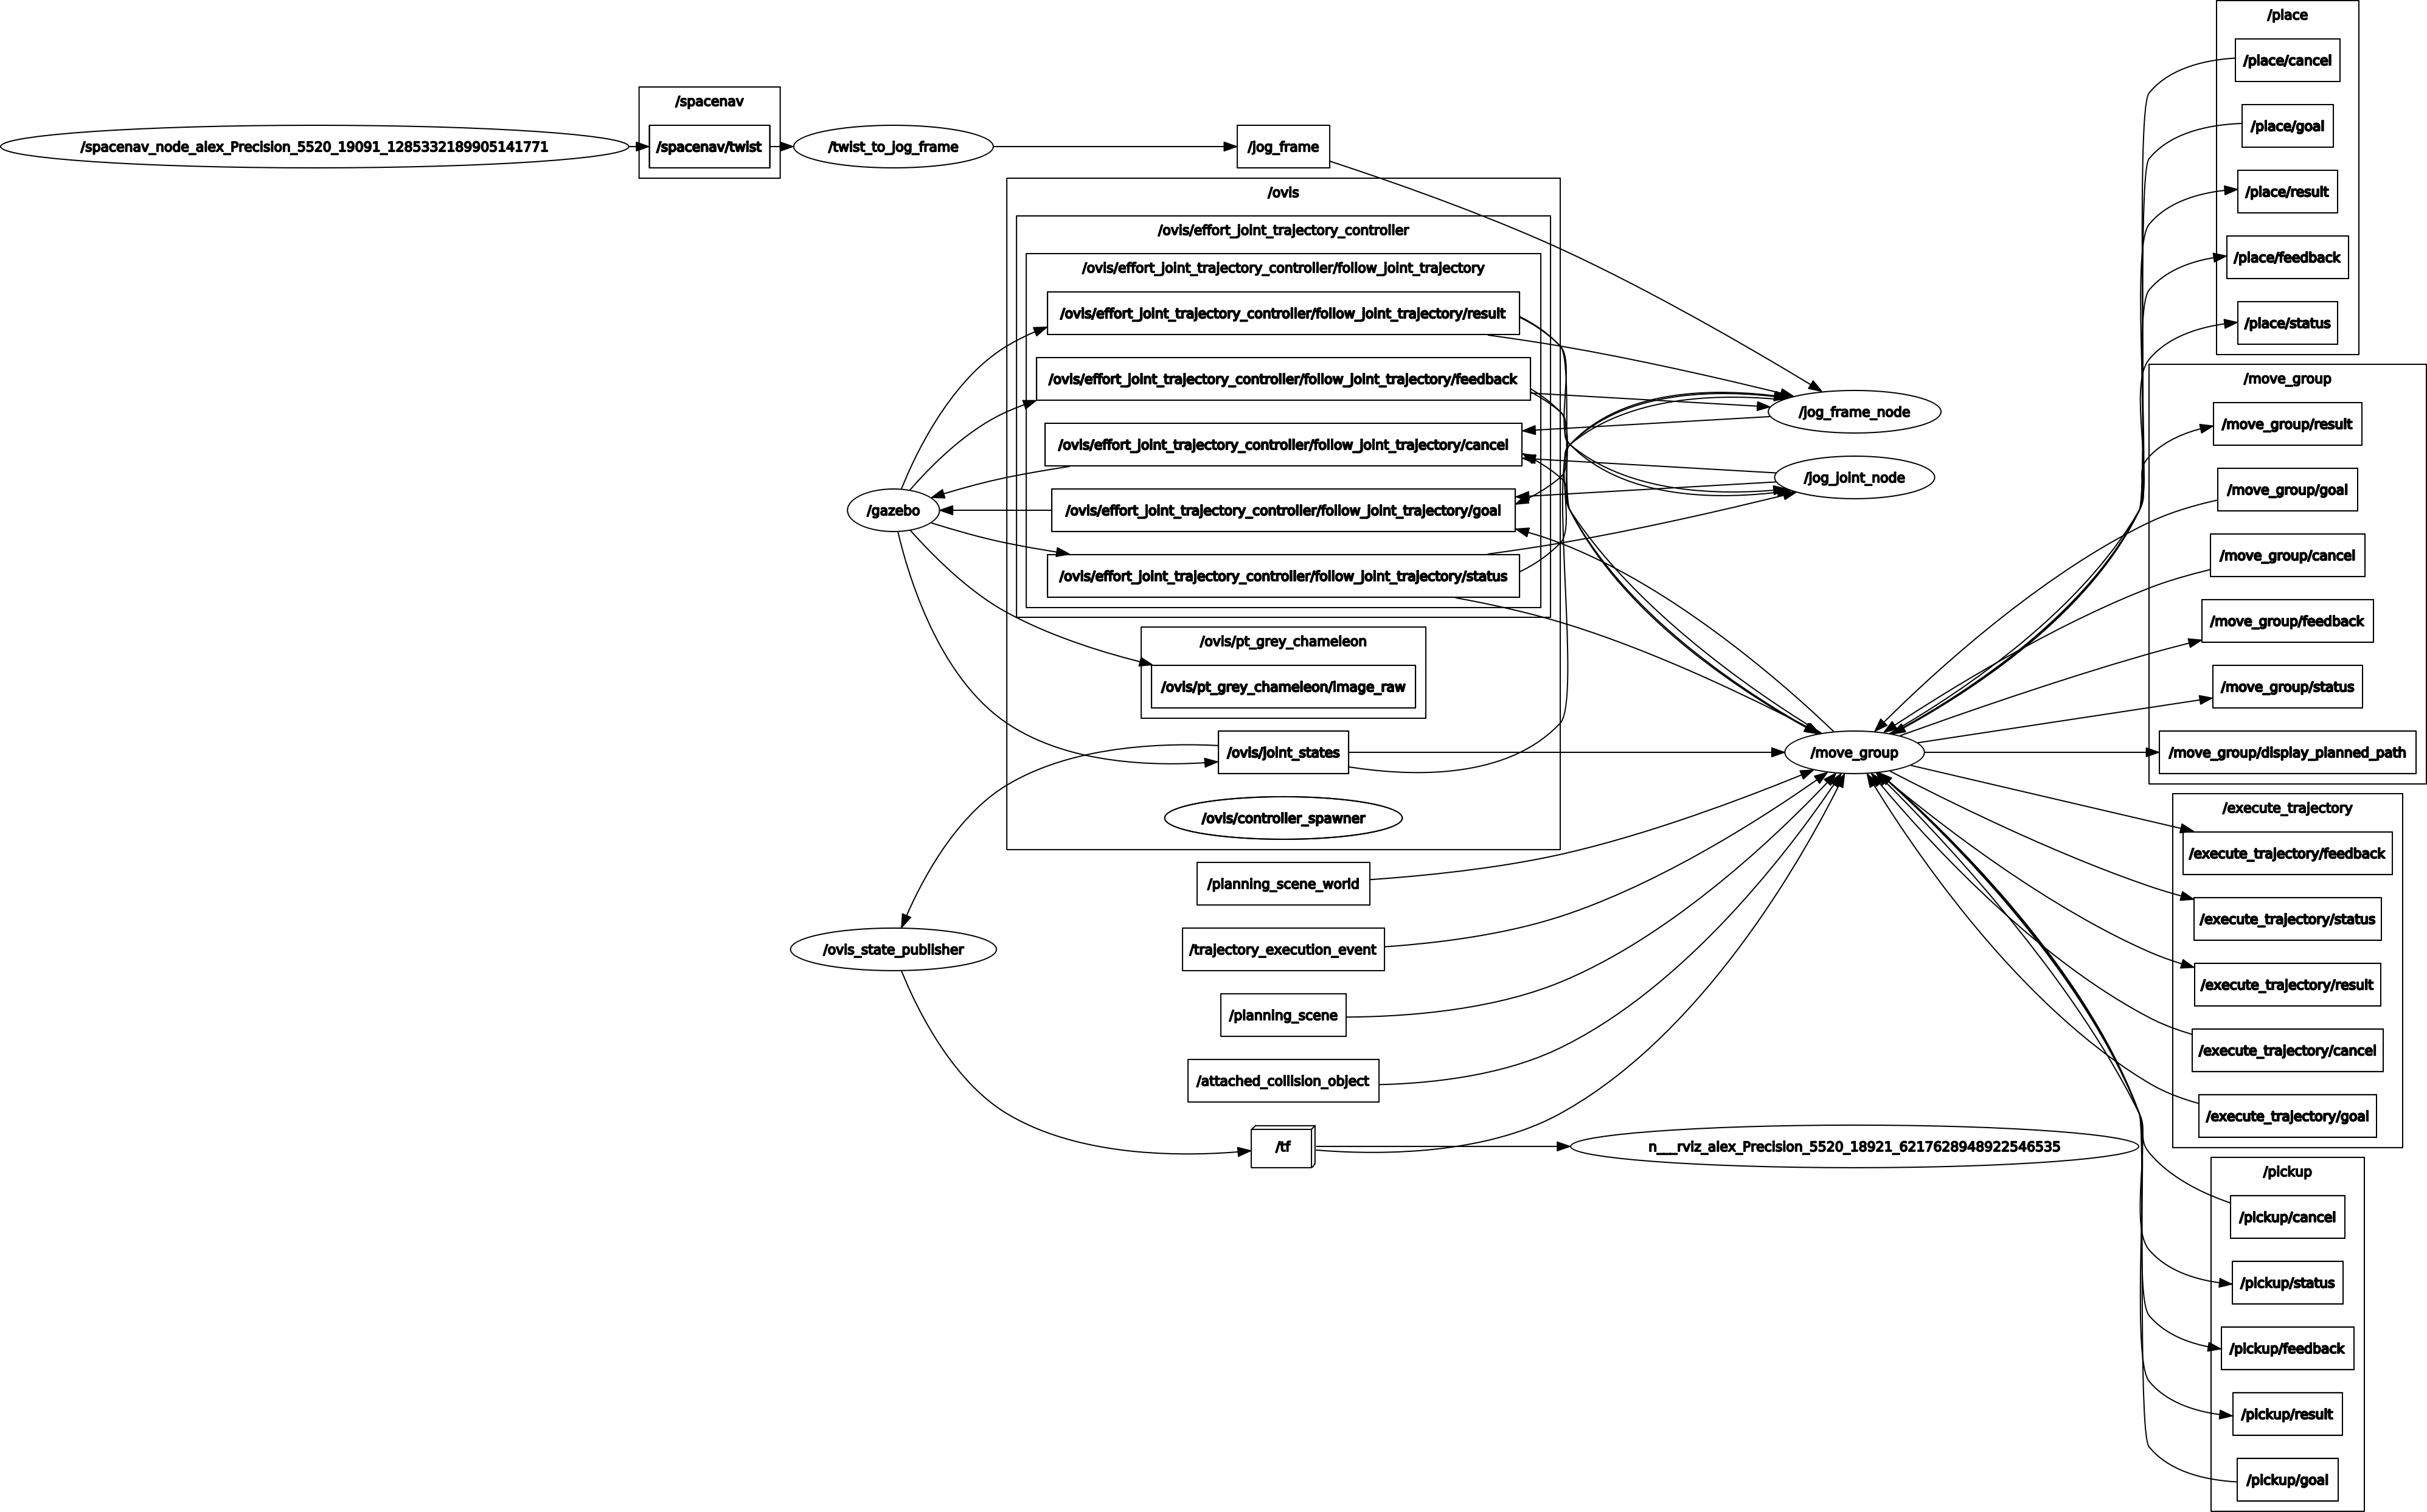
\includegraphics[%scale=0.35
                    width=\textwidth]{Figures/ovis_rosgraph_sim.png}
    \caption{Liaisons entre les différents noeuds logiciel de la solution}
    \label{fig:rosgraph_sim}
\end{figure}

\section{Interface matériel logiciel}
La communication entre le logiciel et le matériel n'est pas au point. L'ordinateur est apte à communiquer avec le contrôleur Kinova, ceci fut validé par l'envoi de commandes au travers du \emph{UI} fourni par Kinova. Toutefois, la communication entre le logiciel MoveIt et le contrôleur logiciel fourni par Kinova n'est pas complétée. Le contrôleur logiciel Kinova est détecté par le noeud ROS mais n'est pas détecté par MoveIt. Les causes possibles sont les suivantes: la connexion USB est instable, le nom de \emph{topic} attendu par MoveIt ne correspond pas à celui publié par le \emph{driver} Kinova. Ceci est une tâche de configuration assez ardue puisqu'il n'est pas évident à première vue d'établir tous les liens nécessaires. À titre d'exemple, la figure \ref{fig:rosgraph_sim} montre les liaisons entre les différents noeuds logiciel nécessaires au fonctionnement de la simulation visualisés à l'aide du logiciel rqt\_graph\footnote{\href{http://wiki.ros.org/rqt_graph}{wiki.ros.org/rqt\_graph}}. Malgré que ce point du projet est important pour la participation du club à la compétition. Il n'est pas critique à la validation de ce projet, la simulation étant suffisante à l'évaluation de l'algorithme. Il est important de mentionner que puisque l'algorithme est générique, celui-ci pourrait être testé sur tout autre robot supporté par ROS-Industrial et le logiciel \emph{jog\_control}.

